\chapter{Introduction to XBee}\label{introToXBee}

One of the main characteristics of WSNs is the ability each node has to wirelessly communicate with other nodes. 
During this course we will be doing this with ZigBee protocol compliant radios, like XBee~\cite{faludi2010bws}.

Throughout this section you will be introduced to the different components and code that will allow you to set a basic wireless network with XBee modules.

\section{The XBee module hardware configuration}\label{xbee:hardware}

XBee modules come in different configurations. The one we will be using is called XBee Series 2 with wire antenna as it is shown in Figure~\ref{fig:xbee}.

\begin{figure}[htbp]
  \centering
  
\includegraphics[width=0.4\linewidth]{figures/xbee.eps}
  \caption{XBee Series 2 with wire antenna
  \label{fig:xbee}}
\end{figure}

This device supports different kinds of ZigBee in mesh networking. Its wire antenna provides omnidirectional coverage, or what is the same as saying that its coverage is pretty much the same in all directions when the antenna is straight and perpendicular to the module.

If you flip the XBee, you will be able to see the pins through which it can send/receive data to/from sensors, communicate with Arduino, connection to a power supply and GND (more information about the pins can be found in page 15 of~\cite{faludi2010bws}).

\subsubsection{Preparing the XBee for configuration}

We can access and program the XBee through any terminal application and a USB connection. The \emph{breakout board} shown in Figure~\ref{fig:breakoutBoard} allows us to: $1$) plug the XBee into a breadboard, facilitating the wired connections with other components (including the Arduino); as well as the ability to $2$) establish a USB connection to configure the XBee.

\begin{figure}[htbp]
  \centering
  \includegraphics[width=0.4\linewidth]{figures/breakoutBoard.eps}
  \caption{XBee Explorer board from SparkFun
  \label{fig:breakoutBoard}}
\end{figure}

As the pins on the XBee are separated differently than the holes in the breadboard, every time a configuration or wired connection is needed, the XBee should be placed in the breakout board as shown in Figure~\ref{fig:xbeeAndBreakoutBoard}, and then placed on the breadboard.

\begin{figure}[htbp]
  \begin{center}$
    \begin{array}{cc}
      \includegraphics[width=0.4\linewidth]{figures/xbeeAndBreakoutBoard.eps}\label{xbeeOutside} &
      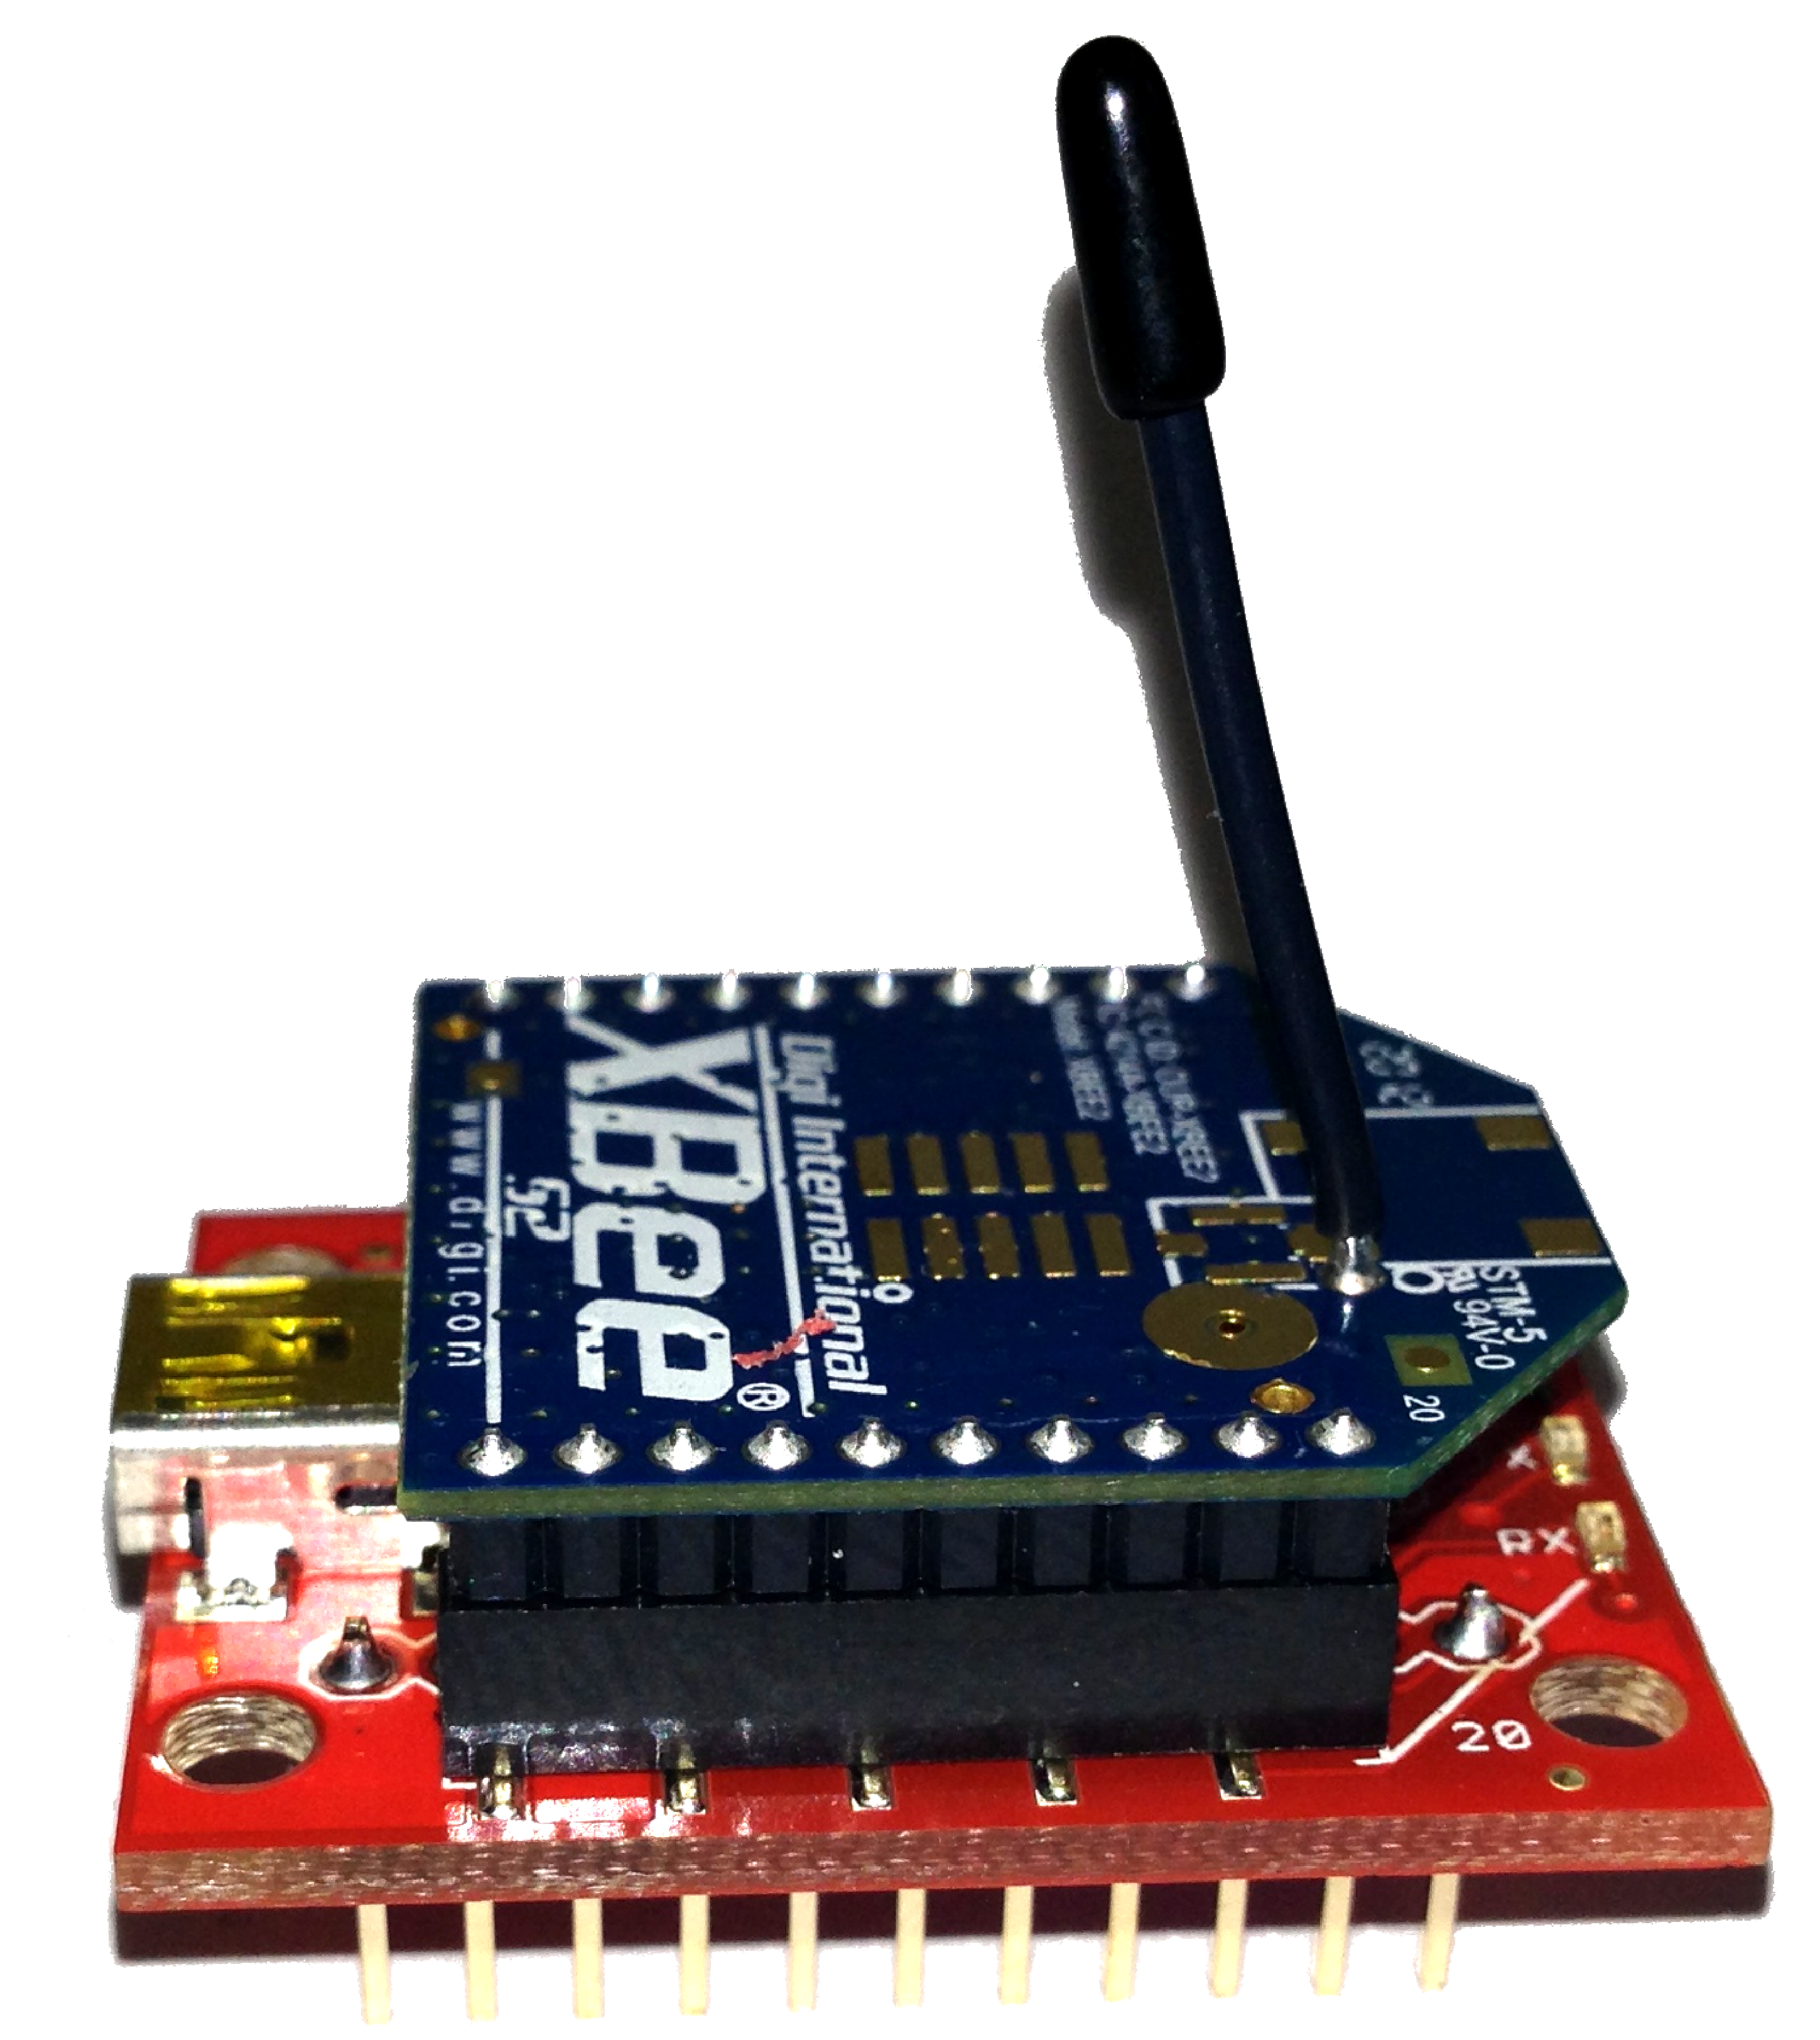
\includegraphics[width=0.4\linewidth]{figures/xbeeAndBreakoutBoard-inserted.eps}\label{xbeeInside}
    \end{array}$
  \end{center}
  \caption{XBee and breakout board: Left: XBee outside; see the different spacing of the pings. Right: XBee inside; setup for configuring and pluging into breadboard.
    \label{fig:xbeeAndBreakoutBoard}}
\end{figure}

It is important to notice that once the XBee is placed on the breakout board, the pins functions change. The new role of each pin is now the displayed underneath the breakout board.

Now that the device is properly placed, we need to setup a connection so the current configuration can be reviewed and changed.

\subsubsection{Accessing the firmware}

The XBee has a microcontroller running a configurable firmware. This firmware holds the necessary information for addressing, communication, security and utility functions. You can configure this firmware to change different settings like: local address, security settings, destination address and how the analog sensors connected to its pins are read.

As for now, the official way to update this firmware is through a program called \emph{X-CTU} and can be downloaded for free from the \emph{\color{blue}{\href{http://www.digi.com/support/kbase/kbaseresultdetl?id=2125}{XBee manufacturer's website}}}.

X-CTU is only available for the Microsoft Windows operating system, nevertheless you have the virtualization option in OS X, as well as WINE Windows emulator in Linux. 

To take a peek at the current XBee configuration: 

\begin{enumerate}
	\item Plug it into one of your computer's USB ports and launch the X-CTU application.
	\item Select the appropriate Com Port listed under \emph{Select Com Port}. This port should be the same in which your XBee is connected.
	\item Confirm that everything is setup correctly by clicking on the \emph{Test/Query} button. If everything is alright, a pop-up window will display the modem type and firmware version.
	\item Change to the \emph{Modem Configuration} tab on the top the X-CTU window. This tab will show you how the firmware is configured.
	\item Under \emph{Modem Parameters and Firmware}, click on the \emph{Read} button. This will fill the current window with the current firmware configuration, as well as the XBee's \emph{Modem} and \emph{Function Set}.
\end{enumerate}

Luckily, X-CTU is only required for upgrading the firmware. For changing the XBee's configuration we only need a USB connection and a terminal software. Nevertheless, this is only possible if the XBee is on \emph{AT command mode} (capable of receiving human commands and forward messages without performing any modification, see Table~\ref{tab:xbeeATModes}). To set it on, follow these steps:

\begin{enumerate}
	\item In the \emph{Model Configuration} tab of the X-CTU, check that the \emph{Modem type} is set to \texttt{XB24-ZB}.
	\item To start, we are going to configure two XBee radios. Under \emph{Function Set}, choose \texttt{ZIGBEE COORDINATOR AT}.
	\item Choose any version greater than \texttt{0x2070}.
	\item Click on the \emph{Write} button to program this device as a coordinator.
\end{enumerate}

Once the installation is complete, gently remove the USB from the first XBee radio a plug it into another. Repeat the process described above, but now under \emph{Function Set} choose \texttt{ZIGBEE ROUTER AT}. Select the highest version available and click on \emph{Write} to program the device.

It is important to distinguish between the two XBee you just configured, given that they behave differently. Every ZigBee network must contain only one coordinator radio, this way the network can be properly defined and managed. Mark which configuration each radio has with a sticker to eliminate any confusion.

\begin{table}[htbp]
	\centering
	\caption{XBee AT modes}
	\label{tab:xbeeATModes}
	\scalebox{0.7}{
	\begin{tabular}{c||c}
		\hline
		\bfseries Transparent mode & \bfseries Command mode\\
		\hline\hline
		Talk \emph{through} the XBee & Talk \emph{to} the XBee itself\\
		Any data can me sent through & Only responds to AT commands\\
		Default state & {\bfseries +++} to enter mode\\
		Wait $10$ seconds to return to this mode & Times out after 10 seconds of no input\\
		\hline
	\end{tabular}}
\end{table}

\subsubsection{Configuring the XBee through a terminal }

There are a lot of terminal applications. Fortunately, most of them need the same kind of information to establish a connection through USB. Table~\ref{tab:terminalParameters} gathers the required settings for a serial terminal software attempting to establish a connection with the XBee.

\begin{table}[htbp]
	\centering
	\caption{Default terminal settings for establishing a connection with an XBee}
	\label{tab:terminalParameters}
	\scalebox{0.7}{
	\begin{tabular}{c||c}
		\hline
		\bfseries Setting & \bfseries Value\\
		\hline\hline
		Baud & $9600$\\
		Data & $8$~bit\\
		Parity & None\\
		Stop bits & $1$\\
		Flow control & None\\
		Line feed & CR+LF or Auto Line Feed\\
		Local echo & on\\
		\hline
	\end{tabular}}
\end{table}

To check if you are already inside the XBee, try asking the radio to go to command mode issuing the \texttt{+++} instruction. If after a moment an \texttt{OK} appears at the right hand side, then you are in!

\subsubsection{Reviewing some AT commands for the XBee}

Issuing commands from a serial connection (like the one you established with the terminal program) to the XBee follows a simple guideline: \emph{instruction parameter} \texttt{<CR>}. Where \texttt{<CR>} accounts for \emph{carriage return}, and just means that you have to press the Return (Enter) key to submit the command. Passing and empty \emph{parameter} just outputs the current value of the specified register (the \emph{instruction} part of the command).

All AT commands start with the \texttt{AT} prefix (accounting for \emph{attention}) and then are followed by a two letter character command identification. Some of the basic AT commands are described below, as well as in~\cite{faludi2010bws}.

\begin{itemize}
	\item \texttt{AT}: gets the attention of the XBee. Its normal output is \texttt{OK}. If you do not receive this output,  you've probably timed out of command mode and need to reissue the \texttt{+++} command to get back in it.
	\item \texttt{ATID}: without any parameter it shows the current Personal Area Network ID (PAN ID) that is assigned to the radio. You can set a PAN ID passing an hexadecimal number in the range $0$x$0$-$0$xFFFF as a parameter.
	\item \texttt{ATSH/ATDL}: it shows the \emph{high} or \emph{low} parts of the unique XBee $64$-bit serial number, respectively. This number cannot be changed, so passing a parameter will produce an \texttt{ERROR} response.
	\item \texttt{ATDH/ATDL}: it shows the \emph{high} or \emph{low} parts of the \underline{destination} address the local radio will forward messages to, respectively. Putting address information after \texttt{ATDH} or \texttt{ATDL} will set the \emph{high} or \emph{low} parts of the destination address, accordingly.
	\item \texttt{ATWR}: saves the current configuration to firmware, so it will become the default configuration the next time you power on the XBee.
\end{itemize}

		